\documentclass[11pt]{report}
 
\usepackage[utf8]{inputenc}
\usepackage[francais]{babel}
\usepackage{fancyhdr}
\usepackage[scale=0.7]{geometry}
\usepackage{lastpage}
\usepackage{titlesec}
\PassOptionsToPackage{hyphens}{url}\usepackage{hyperref}
\usepackage{graphicx}
\usepackage{eurosym}

\newsavebox{\BBbox}
\newenvironment{DDbox}[1]{
\begin{lrbox}{\BBbox}\begin{minipage}{\linewidth}}
{\end{minipage}\end{lrbox}\noindent\colorbox{Zgris}{\usebox{\BBbox}} \\
[.5cm]}

\titleformat{\chapter}[hang]{\bfseries}{\huge\thechapter. }{12pt}{\huge}

\pagestyle{fancy}
\fancyhf{}
\renewcommand{\footrulewidth}{0.4pt}
\renewcommand{\footrulewidth}{0.4pt}
\fancyhead[L]{B engine}
\fancyhead[C]{Projet}
\fancyhead[R]{Groupe B}
\fancyfoot[C]{\textbf{Page \thepage{} sur \pageref{LastPage}}}
\fancyfoot[L]{IUT de Nantes}
\fancyfoot[R]{2014}

\title{Cahier des charges de B engine}
\author{Thibaud \bsc{Courtoison} \\ Dylan \bsc{Gautier} \\ Mathieu \bsc{Grondin} \\ Thomas \bsc{Picard} \\ Hugo \bsc{Pigeon} \\ Maël \bsc{Quémard}}

\makeatletter
\def\maketitle
{
	\begin{titlepage}
		\null\vfill
		\begin{figure}[t]
			\begin{minipage}{0.49\textwidth}
				
\includegraphics[scale=0.5]{iut.jpg}
			\end{minipage}
			\begin{minipage}{0.49\textwidth}
				
\includegraphics[scale=0.5]{univ.jpg}
			\end{minipage}
		\end{figure}
		\begin{center}
			{\LARGE \@title}
			\vskip 1cm
			{\Large \@author}
			\vskip 1cm
			{\Large \@date}
		\end{center}
		\vfill\null
	\end{titlepage}
}
\makeatother

\begin{document}
	\maketitle
	\thispagestyle{empty}

	\chapter{Présentation générale du problème}
	\thispagestyle{fancy}
		\section{Projet}
			\subsection{Finalités}
		
				L’objectif de ce projet est de réaliser un prototype d’un jeu de plateforme en 2D en java se basant sur un moteur de jeu que l’on va faire.
		
			\subsection{Espérance de retour sur investissement}
		
				\begin{itemize}
				  \item Projet Open Source
				  \item Etablissement d’une communauté (github)
				  \item Première expérience dans l’élaboration d’une IHM
				  \item Projet modulaire
				  \item Connaissance sur le développement d’un jeu vidéo et ses contraintes propres
				\end{itemize}
	
		\section{Contexte}
	
			\subsection{Situation du projet par rapport aux autres projets du groupe}
		
				Tous les membres du groupe ont déjà codé le jeu d’Awalé et le jeu du taquin en C en mode console, et nous allons bientôt coder un jeu d’échecs martiens en java. Ces projets nous permettent de connaître l‘utilisation des matrices ainsi que la décomposition des classes d’un jeu.

	Hugo a déjà créé un jeu “snake” en 2D et le langage utilisé dans ce projet est le C++, ce qui représente une certaine expérience de la création d’un jeu avec un langage orienté objet. 
	Thibaud a déjà programmé un “Guitar Hero like” en 2D en java, ainsi qu’un début de Shoot’m up en scrolling horizontal.

			\subsection{Études déjà effectuées}

				\begin{itemize}
				  \item \textbf{Etude des collisions}\\
				  	\url{http://fr.openclassrooms.com/informatique/cours/theorie-des-collisions}\\
				  	Il existe plusieurs types de collisions. Le plus simple et le plus rapide dans son exécution est le AABB. Il s’agit de créer un rectangle autour de chaque entité, les collisions seront détectées à l’intérieur de ce rectangle. On peut également choisir de gérer les collisions au pixel près, mais le traitement est plus lourd. Pour optimiser le traitement, il est possible de diviser la carte du niveau en plusieurs parties et seule la partie contenant le joueur sera traitée.
				  	
				  \item \textbf{Gestion d’une carte ASCII}\\
				  	\url{http://fr.openclassrooms.com/informatique/cours/tile-mapping}\\
		      		Ce tutoriel explique les notions de “Tile mapping”, de “Scrolling” et de déplacement d’un personnage en suivant la gravité. L’avantage de ce tutoriel est qu’il donne des bouts d’algorithmes permettant de comprendre ces notions à un niveau informatique.
		      		
				  \item \textbf{MVC}\\
				  	\url{http://www.u-picardie.fr/~furst/docs/3-%20Event_MVC.pdf}\\
		      		Le MVC (modèle vue contrôleur) consiste à séparer en trois parties les classes d’un programme utilisant une interface graphique. La partie modèle contient toutes les données, la vue consiste à afficher ces données et à détecter les événements (clavier ou souris par exmple). Le contrôleur reçoit les notifications de la vue pour les transmettre au modèle. Cette architecture permet d’avoir un code très modulaire, ont peut facilement créer plusieurs vues sans modifier les autres parties par exemple.
				  	\begin{figure}[h]
		      			\begin{center}
					  		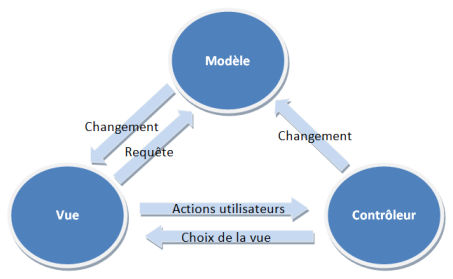
\includegraphics[scale=0.8]{mvc.png}
		      			\end{center}
				  	\end{figure}
				  \item \textbf{Programmation orientée composants}\\
				  	\url{http://perso.citi.insa-lyon.fr/sfrenot/cours/cours01/POO/cours/Composant.pdf}\\
				  	La programmation orientée composants est une technique de programmation plus abstraite que l’orienté objet. Il s’agit de programmer en faisant en sorte que les fichiers compilés soient réutilisables facilement dans d’autres projets. L’objectif est de disposer de programmes très modulaires qui ne diffèrent que par leur implantation.
				\end{itemize}
				
			\subsection{Études menées sur des sujets voisins}
			
				Nous ne menons aucun projet voisin.
				
			\subsection{Suites prévues}
			
				\begin{itemize}
					\item Création d’un éditeur de cartes.
					\item Proposer un export des cartes pour les partager.
					\item Ajout de niveaux dans le jeu.
					\item Ajouter une dimension scénaristique au jeu.
    			\end{itemize}
    			
    		\subsection{Nature des prestations demandées}
    		
    			La prestation demandée est un service, dans le but d’offrir au demandeur un prototype de jeu.
    		
    		\subsection{Parties concernées par le déroulement du projet et ses résultats (demandeurs, utilisateurs)}
    		
    			Le demandeur de ce projet est Adrien Bougouin. Les utilisateurs sont les fans de jeux vidéos rétros.
    		
    		\subsection{Caractère propre à la diffusion}
    		
    			Ce projet sera distribué sous licence Creative Commons avec attribution (\url{http://creativecommons.org/licenses/by/2.0/fr/}) 

				\begin{figure}[h]
		      		\begin{center}
					  	
\includegraphics[scale=0.8]{licence.png}
		      		\end{center}
				 \end{figure}
			
		\section{Énoncé du besoin (finalités du produit pour le futur utilisateur tel que prévu par le demandeur)}
		
			L'objectif de ce projet est de réaliser une première version d'un jeu de plates-formes 2D en Java. Dans cette version, un joueur peut se mouvoir sur des plates-formes.\\

			Afin de faciliter la transition de ce prototype (travail demandé) vers une version multi-joueurs et multi-niveaux (travail non demandé, sauf souhait des étudiants), l'aspect modulaire de l'architecture du jeu est très importante. De même, une réflexion sur les patrons de conception à appliquer est attendue.\\

			Dans le but de valider la modularité de leur architecture, les étudiants doivent proposer deux vues (simultanées) et deux gestionnaires de collisions. Le résultat des vues est similaire, mais visuellement différent :
			\begin{itemize}
			 	\item Affichage 2D classique
			 	\item Affichage textuel du déroulement du jeu
			 \end{itemize}
			 Un gestionnaire de collisions, parmi les deux, est sélectionné au lancement du niveau :
			 \begin{itemize}
				\item Collisions classiques
			 	\item Collisions dans un "monde en caoutchouc"
			 \end{itemize}
			 
			Pour les gestionnaires de collisions, les étudiants doivent s'appuyer sur des algorithmes existants.
		
		\section{Environnement du produit recherché}
		
			\subsection{Listes exhaustives des éléments (personnes, équipements, matières…) et contraintes (environnement)}
			
				6 étudiants : Thibaud \bsc{Courtoison}, Mathieu \bsc{Grondin}, Thomas \bsc{Picard}, Dylan \bsc{Gautier}, Hugo \bsc{Pigeon}, Maël \bsc{Quémard}.
				
				Le jeu sera disponible sur plusieurs OS.
				
				Le jeu sera développé avec le langage de programmation Java
				
				Nous utiliserons des packs graphiques en licences libres.
    		
    		\subsection{Caractéristiques pour chaque élément de l’environnement}
    		
    			\begin{itemize}
    				\item Responsable de l’éditeur de map - Hugo
    				\item Responsable Vue - Dylan
					\item Responsable Modèle - Thomas
					\item Responsable du moteur physique - Mathieu
					\item Responsable Contrôleur - Maël
					\item Responsable Communication Interne/Externe - Thibaud
    			\end{itemize}
    			
    			Le jeu sera disponible sur Linux, Windows et MacOS X.
    			
        		Les packs graphiques suivants seront utilisés pour la conception du jeu :
				 
        		\begin{itemize}
	        		\item UI pack : \url{http://opengameart.org/content/ui-pack}
		      		\begin{center}
					  	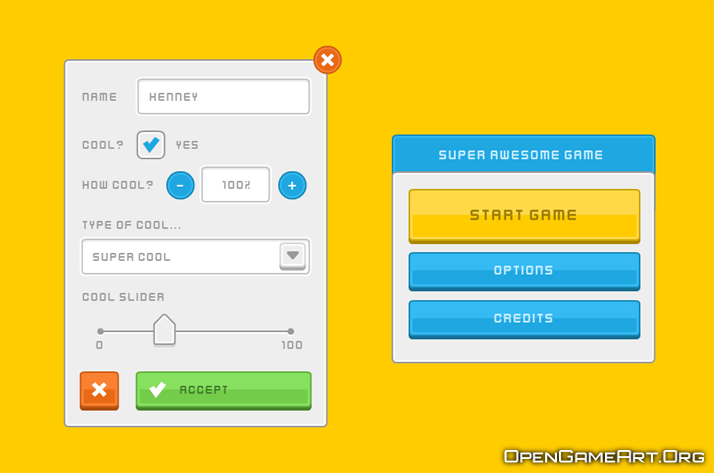
\includegraphics[scale=0.4]{sample_19.png}
		      		\end{center}
					\item Platformer pack : \url{http://opengameart.org/content/platformer-art-complete-pack-often-updated}
		      		\begin{center}
					  	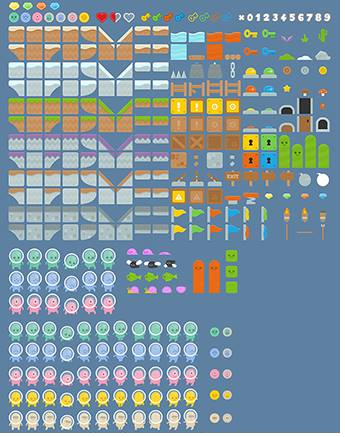
\includegraphics[scale=0.5]{tileset.jpg}
		      		\end{center}
				\end{itemize}
				
	\chapter{Expression fonctionnelle du besoin}
	\thispagestyle{fancy}

		\begin{figure}[h]
		     \begin{center}
			 	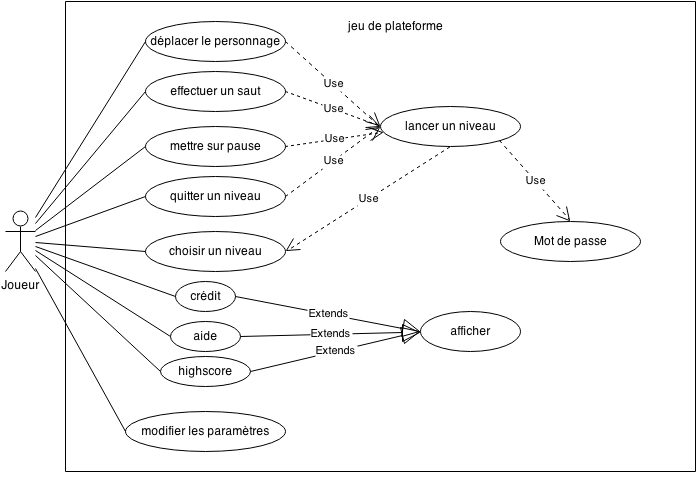
\includegraphics[scale=0.6]{use-case.png}
		     \end{center}
		\end{figure}
		
		\section{Fonctions de service et de contrainte}
		
			\subsection{Fonctions de service principales (qui sont la raison d’être du produit)}
			
				Les services principaux du prototype de jeu sont basés sur :
				\begin{itemize}
			   		\item Un moteur de jeu (modèle MVC)
				    \item Modularité et évolution
				    \item 2 méthodes de collisions (normal et en caoutchouc)
				    \item 2 vues (console + graphique)
				    \item Une carte ascii
            	\end{itemize}
				Exemple de carte ascii :
				\begin{verbatim}
					Tilemapping Version 1.0
					#tileset
					tileset1.bmp
					8 1
					tile0: vide
					tile1: plein
					tile2: plein
					tile3: plein
					tile4: plein
					tile5: plein
					tile6: plein
					tile7: plein
					#level
					15 13
					0 0 0 0 0 0 0 0 0 0 0 0 0 0 0
					0 0 0 0 0 0 0 0 0 0 0 0 0 0 0
					0 0 0 0 0 0 0 0 0 0 0 0 0 0 0
					0 0 0 0 0 0 0 0 0 0 0 0 0 0 0
					1 0 0 0 0 0 0 0 0 1 1 1 1 1 0
					0 0 0 0 0 0 0 0 0 0 0 0 0 0 0
					0 0 0 0 0 0 0 0 0 0 0 0 0 0 0
					0 0 0 0 0 0 0 0 0 0 0 0 0 0 0
					0 0 3 4 0 0 0 2 2 2 2 0 0 2 2
					0 0 5 6 0 0 0 0 0 0 0 0 0 0 0
					0 0 5 6 0 0 0 0 0 0 0 0 0 0 0
					0 0 5 6 0 0 0 0 0 0 0 0 0 0 0
					7 7 7 7 7 7 7 7 7 7 7 7 7 7 7
					#fin
				\end{verbatim}
				
			\subsection{Fonctions de service complémentaires (qui améliorent, facilitent ou complètent le service rendu)}
			
				Parmi les fonctions complémetaires, la conception d’un éditeur de carte ASCII pourrait être un plus à ce projet.
			
			\subsection{Contraintes (limitations à la liberté du concepteur-réalisateur)}
			
				Les graphismes, le nom du jeu et le gameplay ont une limitation imposée.
				
				Utilisation de Github (\url{https://github.com/ErrOrnAmE/S2Game})
			
		\section{Critères d’appréciation (en soulignant ceux qui sont déterminants pour l’évaluation des réponses)}
		
			\begin{itemize}
				\item \underline{Un déplacement fluide}
				\item \underline{Une bonne résolution}
				\item \underline{Présence d’items sur la carte (au moins un)}
				\item \underline{Système de mot de passe pour chaque niveau}
				\item \underline{Un niveau en collision caoutchouc}
				\item \underline{Présence d’un menu}
				\item \underline{Mode console et mode graphique}
				\item Modularité et évolution
				\item La distribution de sources commenté, ainsi qu’une documentation est censée permettre la modularité et une évaluation
				\item Ajout de plusieurs niveaux
				\item Ajout de textures (HD ou rétro)
			\end{itemize}
		
		\section{Niveaux des critères d’appréciation et ce qui les caractérise}
		
			\subsection{Niveaux dont l’obtention est imposée}
			
				La réalisation des fonctionnalités suivantes est imposée :
				\begin{itemize}
					\item Un déplacement fluide
					\item Une bonne résolution
					\item Présence d’items sur la carte (au moins un)
					\item Système de mot de passe pour chaque niveau
					\item Un niveau en collision caoutchouc
					\item Présence d’un menu
					\item Mode console et mode graphique
				\end{itemize}
				
				Nous n’accorderons cependant pas une grande importance au son.
				
			\subsection{Niveaux souhaités mais révisables}
			
				\begin{itemize}
				\item Modularité et évolution
				\item La distribution de sources commenté, ainsi qu’une documentation est censée permettre la modularité et une évaluation
				\item Ajout de plusieurs niveaux
				\item Ajout de textures (HD ou rétro)
				\end{itemize}
	
	\chapter{Cadre de réponse}
	\thispagestyle{fancy}
	
		\section{Pour chaque fonction}
		
			% \subsection{Solution proposée}
			
			% \subsection{Niveau atteint pour chaque critère d’appréciation de cette fonction et modalités de contrôle}
			
			\subsection{Part du prix attribué à chaque fonction}
			
				\textbf{Fonction : temps estimé $\Rightarrow$ coût $\Rightarrow$ rémunération}
				
				Jeu de base: 3 semaines $\Rightarrow$ 7500\euro{} $\Rightarrow$ 1143,60\euro /personne.
				
				Packs de texture: 1 semaine $\Rightarrow$ 500\euro{} $\Rightarrow$ 76,24\euro /personne.
				
				Niveau(x) “caoutchouc”: 1 semaine $\Rightarrow$ 500\euro{} $\Rightarrow$ 76,24\euro /personne.
				
				Nouvelle(s) carte(s) de jeu: 1 semaine $\Rightarrow$ 500\euro{} $\Rightarrow$ 76,24\euro /personne.
				
				Affichage console: 1 semaine $\Rightarrow$ 500\euro{} $\Rightarrow$ 76,24\euro /personne.
				
				Implanter une nouvelle résolution graphique: 1 semaine $\Rightarrow$ 500\euro{} $\Rightarrow$ 76,24\euro /personne.
			
		\section{Pour l’ensemble du produit}
		
			\subsection{Prix de la réalisation de la version de base}
			
				Le prix de réalisation pour la version de base est de 7500\euro{} toutes taxes comprises.
			
			\subsection{Options et variantes proposées non retenues au cahier des charges}
			
				Les options suivantes n’ont pas été retenu au cahier des charges :
				\begin{itemize}
                	\item Possibilité de jouer en résau
		            \item Présence d’une Intelligence Artificielle
		            \item Possibilité de jouer en multijoueur
                \end{itemize}
                
                Nous n’avons pas retenu ces fonctionnalités car leur réalisation nous semble difficile et coûteuse en temps. Nous préfèrons nous concentrer sur les bases du moteur de jeu pour qu’il soit pleinement fonctionnel.
                
			\subsection{Mesures prises pour respecter les contraintes et leurs conséquences économiques}
			
				Le respect des contraintes est évalué par une note de travail.
			
			\subsection{Outils d’installation, de maintenance… à prévoir}
			
				Utilisation de Ant: \url{http://ant.apache.org/}
				
           		Création d’une documentation pour le moteur de jeu
           		
           		Création d’un manuel d’utilisation pour le jeu
           	
           	\subsection{Décomposition en modules, sous-ensembles}
           	
           		Respect des patrons de conception MVC et Observeur/Observable
           		
           	\subsection{Prévisions de fiabilité}
           	
           		Aucune conséquence néfaste pour l’utilisateur ainsi que pour le système.
           	
           	\subsection{Perspectives d’évolution technologie}
           	
           		\begin{itemize}
           			\item Ajout du multijoueur
					\item Multilangue
					\item Mode 18+ (+ de sang, plus de “sous-entendu”)
				    \item Jeu en réseau
				    \item Ajout d’une Intelligence Artificielle
				    \item Génération de map aléatoire
				    \item Ajout d’élément décoratif (nuages)
				    \item Ajout de Warpzones
		        \end{itemize}

\end{document}
